\documentclass{sigchi}
\usepackage{times}
\usepackage{graphicx}
\usepackage{amsmath, amssymb,latexsym}
\usepackage{url}
\usepackage{epstopdf}

%Change the date in \wintitle with the otpinal argument

\newcommand\tabhead[1]{\small\textbf{#1}}

\newcommand{\superscript}[1]{\ensuremath{^{\textrm{#1}}}}
\def\sharedaffiliation{\end{tabular}\newline\begin{tabular}{c}}

\def\winlab{\superscript{\dag}}
\def\cmu{\superscript{$\ast$}}
\def\ut{\superscript{\S}}
\makeatletter
\let\@copyrightspace\relax
\makeatother
%The optional argument for \winstudent is for the number of students
%If the project has only one student, omit the optional argument.



%\numberofauthors{1}
%\author{
%\alignauthor
% Sugang Li\winlab, Ashwin Ashok\cmu, Yanyong Zhang\winlab, Chenren Xu\cmu, Macro Gruteser\winlab, Janne Lindqvist\winlab\\
%\vspace{4mm}
%        \affaddr{{\winlab}WINLAB, Rutgers University, North Brunswick,NJ, USA}\\
%          \vspace{1mm}
%        \affaddr{{\cmu}Carnegie Mellon University, Pittsburgh, PA, USA}\\
%}

%\usepackage{theorem}

\newtheorem{theorem}{Theorem}
\newtheorem{lemma}{Lemma}
\newtheorem{Lemma}{Lemma}
\newtheorem{Proof}{Proof}
\begin{document}
\title{Headsup Google Glass, Log me in!}
\maketitle
\newcommand{\systemname}{{\em MusicMove}}
%%%%%%%%%%%%%%%%%%%
\begin{abstract}
%%%%%%%%%%%%%%%%%%%
In this project, we demonstrate a practical novel approach to authenticate a user on a head-worn device with limited input hardware, by monitoring the user's unique head movement patterns stimulated by an external audio music. Existing solutions today rely on indirect authentication via smartphone or swipe pattern on the built-in touchpad. These could be cumbersome and vulnerable. In the other hand, biometric approach such as fingerprint and iris are subject to the availability of the sensor unit. The proposed system, ~\systemname, addresses these concerns, and provide a practical solution with high authentication accuracy. In average, our system can achieve true acceptance rate of 95.57\% while the false acceptance rate is only 4.43\%.
\end{abstract}


\section{Introduction}
After decades of effort on hardware and battery research, wearable devices become pervasive and an integral part of humans lives~\cite{googleglass,smartwatch,fitbit}. 
%The advances in wearable technology and the ardent interest in gaming and artificial reality have spiked a great consumer interest in the use of head-worn devices~\cite{googleglass,occulusrift,hololens}. 
%Head-worn devices, similar to any 'smart' mobile device today, equip inertial measurement units (IMU) for tracking simple head movements.
%However, through a careful probing into the IMU's accelerometer readings, we identified that, when user's make known head-movement patters such as head banging, nod, lateral shakes, these readings carry a unique pattern for each user; something of a signature type. This motivates us to ask the fundamental question as to {\em why not use such signatures to authenticate users to their head-worn wearable device?}.
 
%Body movement patterns have long been used by humans to discriminate between people. By watching how a person walks, dances, waves hands, we can often recognize the person from afar. A similar rationale applies for head movements. Human body movements are usually \emph{distinctive} and \emph{repeatable}. However, proving the distinctiveness and repeatability based on IMU sensor readings, however, is not straightforward and poses significant signal processing challenges such as classifying different users based on their head-movements captured through such noisy motion sensors. Moreover, it is also not clear what resolution of the sensing is required to capture the movements such that the signatures may be extracted. In addition, the fact that the system must run on a energy and computationally resource constrained wearable device poses significant system design challenges.

\iffalse
Moreover, each device will have only a 
limited view of body movements, dependent on its mounting position on the 
human body. In this project, we set out to conduct a holistic study of wearable 
authentication through body movements and to design an accurate, robust and 
light-weight authentication system. A key distinguishing feature of our work 
is that we will also consider stimuli that wearable devices can provide to 
design challenge-response inspired mechanisms, particularly stimuli that are 
difficult to observe even for the closest adversaries. For example, we can use 
fast-tempo music through earbuds to stimulate movements and to make such 
free-style movements more repeatable. 

In particular, we have designed and implemented  \systemname(Figure~\ref{fig:illustrate}), 
an authentication system that generates a signature from user's 
head-movements. These signatures are used as the behavioral biometric. To 
ensure that the user is proactive in making head-movements we stimulate the 
process by playing a short duration audio track with fast beats. The user in 
response to the rhythm and beats makes head-movements that are captured by the 
accelerometer and processed to
generate and authenticate the user's unique biometric signature. Although we 
use a Google Glass a running example for the wearable device, our design can 
be applied to other head-worn gadgets and any system that can record 
head-movements through motion sensing. Our choice for using head movements is 
motivated by the fact that head-worn wearables are becoming very common today 
and such devices are already equipped with motion sensors; for example, 
personal imaging and heads-up display devices, gaming headsets, artificial 
intelligence devices.
\fi

\iffalse
\section{System Design}
We envision that our proposed system will be used as an authentication
interface on the smart-glass wearable device.
The system will run as a service in the device upon power-up,
similar to the screen-lock in smartphones or the head-nod interface on Google
Glass~\cite{googleglass}. Upon usage, a short duration audio track
will be played on the device, and the user makes head-movements in
response to the audio. Our design is developed based on
the idea that humans respond to music naturally through head movements, and that such movements are more
significant and unique when the track contains fast beats and/or rhythm.
\systemname~ generates unique features from the head
movements of a user, and uses them as a biometric signature for
authenticating the right user to the device. The system will
grant access only when the head-movement signature
generated during the login attempt matches with the
original user's signature.

As illustrated in Figure~\ref{fig:sysarch}, the design of the \systemname~ involves the following key steps:
\begin{itemize}
\item {\em Sensor data collection}: The \systemname~records the head-movements
in the form of raw accelerometer signals using the inbuilt accelerometer
sensor on the smart-glass device.
\item {\em Filtering}: The accelerometer signals are filtered by applying
a simple low-pass filter to remove records of extraneous motion.
\item {\em Signature generation}: The accelerometer signals are
processed through the dynamic-time warping (DTW) tool~\cite{dtw} to obtain a
DTW
feature that is treated as the unique signature for the user.
A user can generate different signatures for different audio tracks. A
training phase collects the set of signature for each user-audio pair.
\item {\em Classification}: The signatures are classified as a match or
not a match, based on a thresholding scheme and using the
trained data set as a reference. The system grants the user
access to the device if there is a match with sufficient confidence.
\end{itemize}
\begin{figure}[t]
\centering
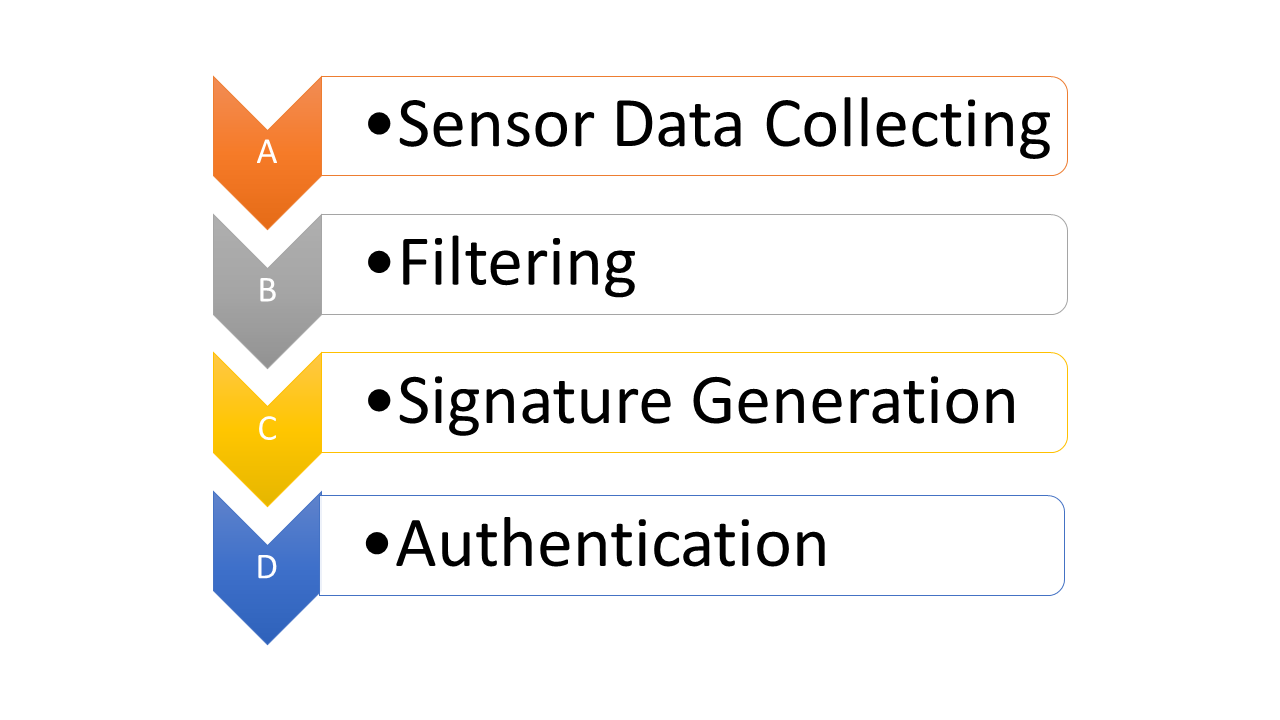
\includegraphics[width=\columnwidth]{pic/workflow.png}
\caption{\systemname~system design flow}
\label{fig:sysarch}
\end{figure}

\fi

\section{What we have implemented}

\begin{figure}[t]
\centering
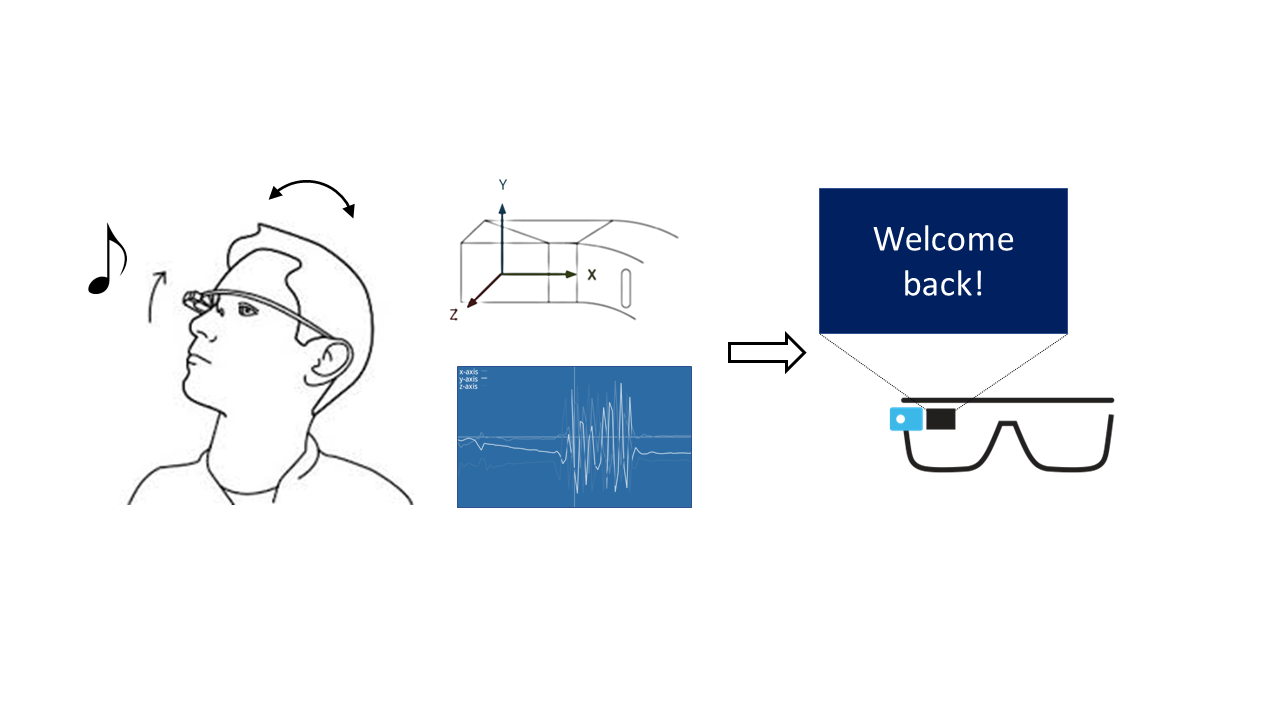
\includegraphics[width=\columnwidth]{pic/headbanger_illustrate.png}
\caption{\label{fig:illustrate} Illustration of our prototype system for logging in Google Glass through head movements}
\end{figure}

Motivated by possibility of identifying signatures in head-movements we set our foray into implementing a software framework on Google Glass that would enable logging in users to the device through head-nod patterns.
A illustrated in Figure~\ref{fig:illustrate}, we implemented an Android app on Google glass that takes extracts signatures from a user's head-nod pattern and attempts to log in the user using the signature as a feature template. To ensure that we have a sense of the timing in the periodic head-movements we play rhythmic beats (through the app) to which the user responds in the form of periodic head-nod movements. The head-movements, however, can also be recorded subconsciously.
We use dynamic-time-warping (DTW)~\cite{dtw} measure to extract the signature from the head-movements.

\iffalse
app. Upon initiation by the user, the app plays a music cue for a stipulated 
duration. The user conducts head-movements in synchrony with the music cue 
while the app records the accelerometer sensor in parallel. At the end of the 
music cue duration the app executes the data processing phase where the 
sensor readings are input to the \systemname's software modules for 
processing. The processing stage includes the filtering of the accelerometer 
sensor values, classification and feature extraction using DTW, and threshold 
based matching of the generated features with those from training set.
%\systemname extracts the head-movement features through 
%the thresholding process discussed in section~\ref{sec:design}, and compare 
%with the feature templates generated from the training phase. 
Upon completion of data processing, the app responds with a YES or NO textual 
output on the Google Glass screen, depending on match score.

%\begin{figure}[t]
%\centering
%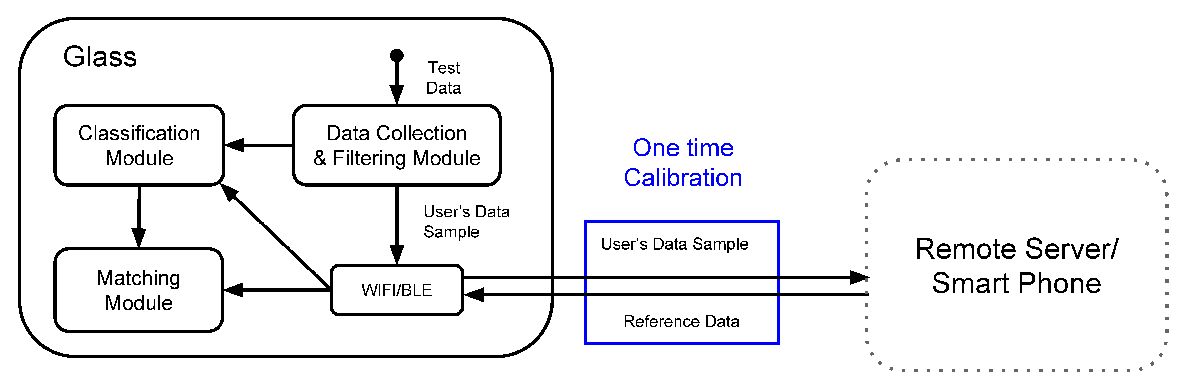
\includegraphics [width=\columnwidth]{pic/software_arch.eps}
%\caption{Software modules of \systemname~implementation}
%\vspace{25 pt}
%\label{fig:glass-softwarearch}
%\end{figure}

In our current implementation, the training phase is conducted offline, prior 
to live-testing off the application.
The training phase involves collecting 30 samples (variable) of the 
head-movement accelerometer readings, generating the features, and saving them 
into a local server (running on PC) as an XML file, with appropriate indexing. 
Upon app initiation on Glass, the trained features are pre-fetched from 
the server through a wireless connection. This ensures that the training set 
is readily available during the authentication process, thus eliminating the 
additional processing time required for the training phase.
Conducting online training, particularly that involves DTW computations, is 
very compute intensive on a resource constrained devices such as Glass. 
One possible solution would be for the Glass to offload the 
training phase computation to a local server machine.
\fi

\section{What we will demonstrate}
%We expect to use the demo opportunity to show the proof-of-concept of \systemname~and absorb the valuable feedback from the researchers. Prior to the demo session, we will pre-load the reference data and parameter of a user. 
During the demo session, the demonstrator will perform head-nod movements by following the music cue (beats) played on the Google Glass device and show the feasibility of our system to login through such head movements.
We will also involve audience participation, where we let the users wear the Google Glass running our login app. We will demonstrate what kind of signatures each user generates when performing the similar head movements and how sensing of such signatures will disallow the users from logging in unauthorized users.
%The authentication result will be presented on the completion of the movement. The user of the Glass will then perform his movement to unlock the device.
%\section{Conclusion}
%\systemname~is an authentication system that can utilize user's head movement under music stimulation . A light-weight algorithm  make it feasible for resource-constraint wearable device. Finally, since it doe s not require additional specific sensor, any  head-worn device can adopt this approach easily.   
\bibliographystyle{unsrt}
\bibliography{sugang}
\end{document}
